\documentclass[12pt,a4paper]{article}

% ─── Page Layout ───────────────────────────────────────────────────────────────
\usepackage[a4paper, margin=0.8in, headheight=14pt]{geometry}

% ─── Fonts (XeLaTeX) ───────────────────────────────────────────────────────────
\usepackage{fontspec}
\usepackage{unicode-math}
\setmainfont{TeX Gyre Pagella}
\setmonofont[Scale=0.88]{TeX Gyre Cursor}
\setmathfont{Latin Modern Math}

% ─── Packages ──────────────────────────────────────────────────────────────────
\usepackage{xcolor}
\usepackage{colortbl}
\usepackage{titlesec}
\usepackage{enumitem}
\usepackage{tabularx}
\usepackage{booktabs}
\usepackage{array}
\usepackage{amsmath}
\usepackage{tikz}
\usetikzlibrary{shapes.geometric, arrows.meta, positioning, calc, fit, decorations.pathreplacing, patterns}
\usepackage[american]{circuitikz}
\usepackage{tcolorbox}
\tcbuselibrary{skins, breakable}
\usepackage{hyperref}
\usepackage{fancyhdr}
\usepackage{graphicx}
\usepackage{microtype}
\hyphenpenalty=10000
\exhyphenpenalty=10000
\sloppy
\usepackage{caption}
\usepackage{setspace}
\usepackage{multirow}
\usepackage{tocloft}

% ─── Q&A helper ────────────────────────────────────────────────────────────────
\newcommand{\Q}[1]{\textbf{#1}\par\noindent\ignorespaces}

% ─── Colour Palette ────────────────────────────────────────────────────────────
\definecolor{myred}{RGB}{196,30,58}
\definecolor{mydark}{RGB}{30,30,50}
\definecolor{mygreen}{RGB}{14,120,80}
\definecolor{myteal}{RGB}{0,130,140}
\definecolor{myamber}{RGB}{180,100,0}
\definecolor{mypurple}{RGB}{100,30,160}
\definecolor{mygray}{RGB}{246,247,249}
\definecolor{mgframe}{RGB}{180,185,200}
\definecolor{watermark}{RGB}{145,150,170}
\definecolor{hdrred}{RGB}{250,232,235}
\definecolor{hdrgreen}{RGB}{220,244,233}
\definecolor{hdrteal}{RGB}{220,242,244}
\definecolor{hdramber}{RGB}{253,242,215}
\definecolor{hdrpurple}{RGB}{238,228,255}
\definecolor{hdrgray}{RGB}{238,240,245}
\definecolor{rowalt}{RGB}{250,251,253}

% ─── Section Formatting ────────────────────────────────────────────────────────
\titleformat{\section}{\large\bfseries\color{myred}}{\thesection.}{0.5em}{}[\vspace{1pt}{\color{myred}\rule{\linewidth}{0.8pt}}]
\titleformat{\subsection}{\normalsize\bfseries\color{myteal}}{\thesubsection}{0.5em}{}
\titlespacing*{\section}{0pt}{18pt}{7pt}
\titlespacing*{\subsection}{0pt}{11pt}{4pt}

% ─── Paragraph ─────────────────────────────────────────────────────────────────
\setlength{\parindent}{0pt}
\setlength{\parskip}{4pt}

% ─── TOC Styling ───────────────────────────────────────────────────────────────
\renewcommand{\cfttoctitlefont}{\large\bfseries\color{myred}}
\renewcommand{\cftaftertoctitle}{\par\noindent{\color{myred}\rule{\linewidth}{0.8pt}}}
\setlength{\cftbeforetoctitleskip}{0pt}
\setlength{\cftaftertoctitleskip}{6pt}
\renewcommand{\cftsecfont}{\normalsize\bfseries\color{mydark}}
\renewcommand{\cftsecpagefont}{\normalsize\bfseries\color{mydark}}
\renewcommand{\cftsecleader}{\cftdotfill{\cftdotsep}}
\setlength{\cftbeforesecskip}{7pt}
\renewcommand{\cftsubsecfont}{\small\color{mydark}}
\renewcommand{\cftsubsecpagefont}{\small\color{mydark}}
\setlength{\cftbeforesubsecskip}{3pt}
\setlength{\cftsubsecindent}{1.4em}

% ─── Table helpers ─────────────────────────────────────────────────────────────
\renewcommand{\arraystretch}{1.45}
\setlength{\tabcolsep}{6pt}
\arrayrulecolor{mydark}
\newcolumntype{B}[1]{>{\small\bfseries\raggedright\arraybackslash}m{#1}}
\newcolumntype{Y}{>{\small\raggedright\arraybackslash}X}
\renewcommand{\tabularxcolumn}[1]{m{#1}}

% ─── Header / Footer ───────────────────────────────────────────────────────────
\pagestyle{fancy}
\fancyhf{}
\fancyhead[L]{\small\color{myred}\textbf{PE-EC802A}\;\color{mydark}--- Mixed Signal Design}
\fancyhead[R]{\small\color{myteal}\textbf{Module 5 Notes}}
\fancyfoot[C]{\small\color{mydark}\thepage}
\fancyfoot[R]{\small\color{watermark}\textit{\copyright\ Biraj}}
\renewcommand{\headrulewidth}{0.5pt}
\renewcommand{\footrulewidth}{0.3pt}

% ─── Hyperref ──────────────────────────────────────────────────────────────────
\hypersetup{colorlinks=true, linkcolor=myteal, urlcolor=myteal,
  pdfauthor={Biraj Sarkar}, pdftitle={PE-EC802A --- Module 5 Notes}}

% ─── tcolorbox styles ──────────────────────────────────────────────────────────
\tcbset{
  tikzbox/.style={colback=mygray, colframe=mgframe, boxrule=0.6pt, arc=4pt,
    left=8pt, right=8pt, top=6pt, bottom=6pt,
    colbacktitle=mgframe, coltitle=mydark, fonttitle=\small\bfseries},
  defbox/.style={colback=hdrgreen, colframe=mygreen, boxrule=0.8pt, arc=4pt,
    left=9pt, right=9pt, top=6pt, bottom=6pt,
    colbacktitle=mygreen, coltitle=white, fonttitle=\small\bfseries},
  formulabox/.style={colback=hdrteal, colframe=myteal, boxrule=0.8pt, arc=4pt,
    left=9pt, right=9pt, top=7pt, bottom=7pt,
    colbacktitle=myteal, coltitle=white, fonttitle=\small\bfseries},
  examplebox/.style={colback=hdramber, colframe=myamber, boxrule=0.8pt, arc=4pt,
    left=9pt, right=9pt, top=6pt, bottom=6pt,
    colbacktitle=myamber, coltitle=white, fonttitle=\small\bfseries},
  masonbox/.style={colback=hdrpurple, colframe=mypurple, boxrule=0.8pt, arc=4pt,
    left=9pt, right=9pt, top=6pt, bottom=6pt,
    colbacktitle=mypurple, coltitle=white, fonttitle=\small\bfseries},
  exambox/.style={colback=hdrpurple, colframe=mypurple, boxrule=1pt, arc=5pt,
    left=10pt, right=10pt, top=8pt, bottom=8pt,
    colbacktitle=mypurple, coltitle=white, fonttitle=\bfseries,
    breakable, title after break={\textbf{Frequently Asked / Viva Questions (contd.)}}}
}
\tcbset{breakable}

% ─── TikZ styles ───────────────────────────────────────────────────────────────
\tikzset{
  block/.style={rectangle, draw=myteal, fill=hdrteal,
    text width=2.4cm, align=center, minimum height=0.95cm,
    font=\small, rounded corners=3pt, line width=0.7pt},
  redblock/.style={rectangle, draw=myred, fill=hdrred,
    text width=2.4cm, align=center, minimum height=0.95cm,
    font=\small, rounded corners=3pt, line width=0.7pt},
  sumjunc/.style={circle, draw=myamber, fill=hdramber,
    minimum size=0.62cm, font=\small, line width=0.8pt},
  arrow/.style={-Stealth, thick, color=mydark},
  line/.style={thick, color=mydark}
}

% ═══════════════════════════════════════════════════════════════════════════════
\begin{document}
% ═══════════════════════════════════════════════════════════════════════════════

\begin{center}
  {\LARGE\bfseries\color{myred} PE-EC802A --- Mixed Signal Design}\\[5pt]
  {\normalsize\color{mydark} Semester VIII \quad$\bullet$\quad 3L:0T:0P \quad$\bullet$\quad 3 Credits}\\[3pt]
  {\normalsize\color{myteal}\textbf{Module 5 Exam Notes}}\\[3pt]
  {\small\color{mydark} CGEC \;$|$\; B.Tech ECE (2023--27) \;$|$\; \textit{Biraj Sarkar}}
\end{center}
\vspace{2pt}
\noindent{\color{myred}\rule{\linewidth}{1.5pt}}
\vspace{2pt}

\hypersetup{linkcolor=mydark}
\tableofcontents
\hypersetup{linkcolor=myteal}
\newpage

% ===============================================================================
\section{Phase-Locked Loop (PLL) Architecture \& Working}
% ===============================================================================

\begin{tcolorbox}[defbox, title={\textbf{Phase-Locked Loop (PLL) Concept}}]
A \textbf{Phase-Locked Loop (PLL)} is a feedback control system that generates an output signal whose phase is locked to the phase of an input reference signal. In mixed-signal systems, PLLs are widely used for frequency synthesis, clock recovery, and jitter reduction.
\end{tcolorbox}

\subsection{Block Components and Signal Flow}
A Charge-Pump Phase-Locked Loop (CP-PLL) consists of five main blocks:

\begin{tcolorbox}[tikzbox, title={Block Diagram of a Charge-Pump PLL}]
\centering
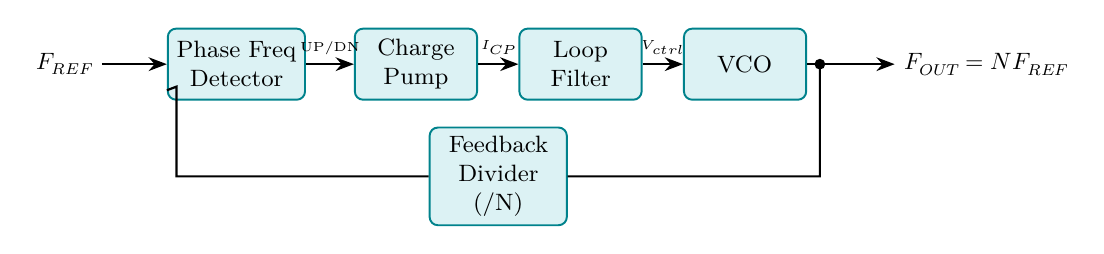
\begin{tikzpicture}[scale=0.95, transform shape]
  % PFD
  \node[block, text width=1.6cm] (pfd) at (0, 0) {Phase Freq\\Detector};
  
  % CP
  \node[block, text width=1.4cm] (cp) at (2.4, 0) {Charge\\Pump};
  
  % LF
  \node[block, text width=1.4cm] (lf) at (4.6, 0) {Loop\\Filter};
  
  % VCO
  \node[block, text width=1.4cm] (vco) at (6.8, 0) {VCO};
  
  % Divider
  \node[block, text width=1.6cm] (div) at (3.5, -1.5) {Feedback\\Divider (/N)};

  % Paths
  \draw[-Stealth, thick] (-1.8, 0) node[left, font=\small] {$F_{REF}$} -- (pfd);
  \draw[-Stealth, thick] (pfd) -- (cp) node[midway, above, font=\tiny] {UP/DN};
  \draw[-Stealth, thick] (cp) -- (lf) node[midway, above, font=\tiny] {$I_{CP}$};
  \draw[-Stealth, thick] (lf) -- (vco) node[midway, above, font=\tiny] {$V_{ctrl}$};
  \draw[-Stealth, thick] (vco) -- (8.8, 0) node[right, font=\small] {$F_{OUT} = N F_{REF}$};
  
  % Feedback path
  \draw[thick] (7.8, 0) to[short, *-] (7.8, -1.5) -- (div);
  \draw[thick] (div) -| (-0.8, -0.8) -- (-0.8, -0.3) -- (pfd);
\end{tikzpicture}
\end{tcolorbox}

\textbf{Working of Each Block:}
\begin{enumerate}[label=\textbf{\arabic*.}, leftmargin=*, itemsep=3pt]
  \item \textbf{Phase Frequency Detector (PFD):} Compares the reference clock $F_{REF}$ with the feedback clock $F_{FB}$. It generates digital pulses (UP and DN) whose widths are proportional to the phase and frequency difference between the inputs.
  \item \textbf{Charge Pump (CP):} Converts the digital UP/DN control pulses into a proportional current charge injection:
  \[
  I_{avg} = I_{CP} \frac{\Delta \Phi}{2\pi}
  \]
  \item \textbf{Loop Filter (LF):} A passive low-pass filter (usually a resistor $R$ in series with a capacitor $C_1$, in parallel with a smaller capacitor $C_2$). It integrates the CP current to generate a smooth analog tuning voltage $V_{ctrl}$.
  \item \textbf{Voltage Controlled Oscillator (VCO):} A circuit whose output frequency is controlled by $V_{ctrl}$. The output frequency is:
  \[
  \omega_{out} = \omega_{fr} + K_{VCO} V_{ctrl}
  \]
  where $\omega_{fr}$ is the free-running frequency and $K_{VCO}$ is the VCO gain (rad/s/V).
  \item \textbf{Feedback Divider (/N):} Divides the high output frequency down to the reference frequency, allowing the loop to lock at $F_{OUT} = N F_{REF}$.
\end{enumerate}

\subsection{Mathematical Loop Dynamics (Type-II CP-PLL)}
A Type-II PLL has two integrators in the loop: the VCO (which integrates frequency to phase: $\Phi_{out} = \int \omega_{out} dt \Rightarrow H_{VCO}(s) = K_{VCO}/s$) and the loop filter (which contains an integrating capacitor).

\textbf{Transfer Functions of Components:}
\begin{itemize}[leftmargin=*, itemsep=2.5pt]
  \item PFD/CP Gain: $K_d = \frac{I_{CP}}{2\pi}$ (A/rad).
  \item Loop Filter Impedance: $Z_{LF}(s) = R + \frac{1}{s C_1} = \frac{1 + s R C_1}{s C_1}$ (ignoring the small parallel capacitor $C_2$).
  \item VCO Transfer Function: $H_{VCO}(s) = \frac{K_{VCO}}{s}$.
\end{itemize}

\textbf{Open-Loop Gain $A(s)$:}
\[
A(s) = K_d \cdot Z_{LF}(s) \cdot \frac{H_{VCO}(s)}{N} = \left(\frac{I_{CP}}{2\pi}\right) \left(\frac{1 + s R C_1}{s C_1}\right) \left(\frac{K_{VCO}}{s}\right) \frac{1}{N}
\]
\[
A(s) = \frac{I_{CP} K_{VCO} (1 + s R C_1)}{2\pi N C_1 s^2}
\]

\textbf{Closed-Loop Transfer Function $H_{cl}(s) = \frac{\Phi_{out}(s)}{\Phi_{in}(s)}$:}
\[
H_{cl}(s) = \frac{N \cdot A(s)}{1 + A(s)} = \frac{\frac{I_{CP} K_{VCO} R}{2\pi} s + \frac{I_{CP} K_{VCO}}{2\pi C_1}}{s^2 + \frac{I_{CP} K_{VCO} R}{2\pi N} s + \frac{I_{CP} K_{VCO}}{2\pi N C_1}}
\]

Comparing this with the standard second-order system denominator $s^2 + 2\zeta\omega_n s + \omega_n^2$:
\begin{tcolorbox}[formulabox, title={\textbf{Type-II CP-PLL Dynamics}}]
\textbf{Natural Frequency ($\omega_n$):}
\[
\omega_n = \sqrt{\frac{I_{CP} K_{VCO}}{2\pi N C_1}}
\]
\textbf{Damping Factor ($\zeta$):}
\[
\zeta = \frac{R C_1}{2} \omega_n = \frac{R}{2} \sqrt{\frac{I_{CP} K_{VCO} C_1}{2\pi N}}
\]
\end{tcolorbox}
The resistor $R$ is critical; it introduces a zero in the open-loop transfer function, stabilizing the second-order feedback loop by providing adequate phase margin (damping).

% ===============================================================================
\section{Delay-Locked Loop (DLL) Architecture \& Working}
% ===============================================================================

\begin{tcolorbox}[defbox, title={\textbf{Delay-Locked Loop (DLL) Concept}}]
A \textbf{Delay-Locked Loop (DLL)} is a feedback system that aligns the phase of an output clock with an input clock by controlling the delay of a Voltage-Controlled Delay Line (VCDL). Unlike a PLL, a DLL does not use an oscillator (VCO); it only shifts the phase of an existing clock.
\end{tcolorbox}

\subsection{Block Components and Signal Flow}
A DLL consists of a Phase Detector (PD), a Charge Pump (CP), a Loop Filter (LF), and a Voltage-Controlled Delay Line (VCDL).

\begin{tcolorbox}[tikzbox, title={Block Diagram of a Delay-Locked Loop}]
\centering
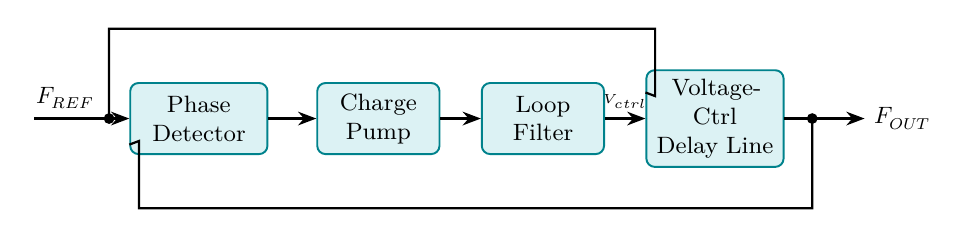
\begin{tikzpicture}[scale=0.95, transform shape]
  % PD
  \node[block, text width=1.6cm] (pd) at (0, 0) {Phase\\Detector};
  
  % CP
  \node[block, text width=1.4cm] (cp) at (2.4, 0) {Charge\\Pump};
  
  % LF
  \node[block, text width=1.4cm] (lf) at (4.6, 0) {Loop\\Filter};
  
  % VCDL
  \node[block, text width=1.6cm] (vcdl) at (6.9, 0) {Voltage-Ctrl\\Delay Line};

  % Paths
  \draw[-Stealth, thick] (-2.2, 0) -- (pd);
  \node[above, font=\small] at (-1.8, 0) {$F_{REF}$};
  \draw[thick] (-1.2, 0) to[short, *-] (-1.2, 1.2) -- (6.1, 1.2) -- (6.1, 0.3) -- (vcdl);
  
  \draw[-Stealth, thick] (pd) -- (cp);
  \draw[-Stealth, thick] (cp) -- (lf);
  \draw[-Stealth, thick] (lf) -- (vcdl) node[midway, above, font=\tiny] {$V_{ctrl}$};
  
  \draw[-Stealth, thick] (vcdl) -- (8.9, 0) node[right, font=\small] {$F_{OUT}$};
  
  % Feedback path
  \draw[thick] (8.2, 0) to[short, *-] (8.2, -1.2) -| (-0.8, -0.6) -- (-0.8, -0.3) -- (pd);
\end{tikzpicture}
\end{tcolorbox}

\subsection{PLL vs. DLL Stability \& Jitter Comparison}

\begin{tcolorbox}[tikzbox, title={Comparison of PLL and DLL Architectures}]
\centering
\par\noindent
\begin{tabularx}{\linewidth}{|B{3.2cm}|Y|Y|}
\hline
\textbf{Parameter} & \textbf{Phase-Locked Loop (PLL)} & \textbf{Delay-Locked Loop (DLL)} \\ \hline
\textbf{Core Component} & VCO (Voltage Controlled Oscillator) & VCDL (Voltage Controlled Delay Line) \\ \hline
\textbf{System Order} & Type-II, 2nd-order or higher (requires series $R$ to stabilize) & Type-I, 1st-order system (unconditionally stable) \\ \hline
\textbf{Jitter Behavior} & \textbf{Jitter Accumulation:} Noise recirculates in the VCO tank/ring, accumulating over cycles & \textbf{No Jitter Accumulation:} Jitter is reset at the end of the delay line every cycle \\ \hline
\textbf{Frequency Synthesis} & Supports frequency multiplication ($F_{OUT} = N F_{REF}$) & Cannot multiply frequency directly; only shifts phase \\ \hline
\textbf{Lock Range} & Limited by VCO tuning range and loop dynamics & Limited by VCDL delay range; prone to harmonic locking \\ \hline
\end{tabularx}
\end{tcolorbox}

\begin{itemize}[leftmargin=*, itemsep=2.5pt]
  \item \textbf{Stability Analysis:} The VCDL is a simple delay stage. Unlike a VCO, it does not integrate frequency to phase (it has no $1/s$ phase term). The DLL closed-loop system is first-order, meaning it is unconditionally stable and the loop filter requires only a single capacitor (no resistor $R$ is needed).
  \item \textbf{Jitter Analysis:} In a VCO, if a clock edge is delayed due to noise, the subsequent edges remain shifted because the phase error accumulates over time. In a VCDL, the input clock is a clean external clock. Any noise-induced delay inside the VCDL affects only the current cycle; the next cycle starts with a fresh, clean reference edge.
\end{itemize}

% ===============================================================================
\section{Digital PLLs \& Frequency Synthesizers}
% ===============================================================================

\subsection{Digital PLL (DPLL) and All-Digital PLL (ADPLL)}
Modern SOCs implement ADPLLs to avoid bulky analog capacitors and process scaling issues:
\begin{itemize}[leftmargin=*, itemsep=2pt]
  \item \textbf{TDC:} A Time-to-Digital Converter replaces the PFD, converting phase differences directly into digital words.
  \item \textbf{Digital Loop Filter (DLF):} Replaces the analog loop filter, saving silicon area and allowing programmable tuning coefficients.
  \item \textbf{DCO:} A Digitally Controlled Oscillator replaces the VCO, using capacitor DAC banks to control oscillation frequency.
\end{itemize}

\subsection{Frequency Synthesizers}
Synthesizers generate multiple frequencies from a single reference:
\begin{itemize}[leftmargin=*, itemsep=2.5pt]
  \item \textbf{Integer-N Synthesizer:} Output frequency is $F_{OUT} = N F_{REF}$. The step size is limited to $F_{REF}$.
  \item \textbf{Fractional-N Synthesizer:} The feedback divider toggles between $N$ and $N+1$ using a Delta-Sigma modulator. This allows the average division ratio to be fractional, providing fine frequency steps with a high reference frequency (reducing loop division noise).
\end{itemize}

% ===============================================================================
% QUICK REVISION PAGE
% ===============================================================================
\newpage
\begin{center}
  {\large\bfseries\color{myred} Quick Revision --- Module 5}\\[3pt]
  {\small\color{mydark} PLLs \& DLLs $|$ PE-EC802A}
\end{center}
\noindent{\color{myred}\rule{\linewidth}{1.2pt}}
\vspace{4pt}

\begin{tcolorbox}[formulabox, title={\textbf{Key Formulas at a Glance}}]
\renewcommand{\arraystretch}{1.35}
\begin{tabularx}{\linewidth}{B{5.0cm} X}
VCO Output Frequency & $\omega_{out} = \omega_{fr} + K_{VCO} V_{ctrl}$ \\[4pt]
PFD/CP Gain & $K_d = \frac{I_{CP}}{2\pi}$ \\[4pt]
VCO Phase integration & $H_{VCO}(s) = \frac{K_{VCO}}{s}$ \\[4pt]
Loop Natural Frequency & $\omega_n = \sqrt{\frac{I_{CP} K_{VCO}}{2\pi N C_1}}$ \\[4pt]
Loop Damping Factor & $\zeta = \frac{R}{2} \sqrt{\frac{I_{CP} K_{VCO} C_1}{2\pi N}}$ \\[4pt]
Integer-N output & $F_{OUT} = N F_{REF}$ \\
\end{tabularx}
\end{tcolorbox}

\begin{tcolorbox}[defbox, title={\textbf{One-Line Definitions}}]
\begin{itemize}[leftmargin=*, itemsep=2pt, topsep=0pt]
  \item \textbf{VCO:} An oscillator whose output frequency is a linear function of its input control voltage.
  \item \textbf{PFD:} A phase-detector block that detects both phase and frequency differences, preventing false lock states.
  \item \textbf{Loop Filter:} A low-pass filter that filters out the high-frequency charge-pump ripple to generate a smooth control voltage.
  \item \textbf{Damping Factor:} A parameter that determines the stability and transient settling time of the PLL loop.
  \item \textbf{VCDL:} A line of buffer stages whose propagation delay is controlled by an input voltage.
  \item \textbf{ADPLL:} A phase-locked loop consisting entirely of digital components (TDC, Digital Filter, DCO).
  \item \textbf{Fractional-N Synthesizer:} A frequency synthesizer that achieves fractional division ratios by dynamically switching divider counts.
\end{itemize}
\end{tcolorbox}

\begin{tcolorbox}[exambox, title={\textbf{Frequently Asked / Viva Questions}}]
\begin{enumerate}[topsep=0pt, label=\textbf{Q\arabic*.}, itemsep=5pt]
  \item \Q{What are the main blocks of a charge-pump PLL?}
    The five main blocks are the Phase Frequency Detector (PFD), Charge Pump (CP), Loop Filter (LF), Voltage-Controlled Oscillator (VCO), and the Feedback Divider (/N).
  \item \Q{Why is a resistor needed in series with the capacitor in a PLL loop filter?}
    The VCO acts as an integrator ($1/s$). If the loop filter is a simple capacitor, it acts as a second integrator ($1/s$). This creates two poles at the origin, making the system unstable (phase margin is $0^\circ$). The resistor introduces a zero ($1+sRC$) that restores stability.
  \item \Q{Compare PLL and DLL stability.}
    A DLL is a first-order system because the VCDL only shifts phase and does not integrate frequency to phase. Therefore, it is unconditionally stable. A PLL is a second-order (or higher) system due to the VCO phase integration and loop filter, requiring careful stabilization.
  \item \Q{Explain the difference in jitter behavior between a PLL and a DLL.}
    In a PLL, phase errors recirculate through the VCO feedback loop, leading to jitter accumulation over time. In a DLL, the input reference clock is clean, and the jitter is reset at the end of the VCDL line every clock cycle, preventing jitter accumulation.
  \item \Q{What is a Phase Frequency Detector (PFD), and what is its advantage over a simple XOR Phase Detector?}
    An XOR PD only detects phase difference and can lock to harmonics or fail to lock if frequencies are different. A PFD detects both phase and frequency differences, ensuring the loop always locks to the correct frequency.
  \item \Q{What is frequency multiplication in a PLL, and how is it achieved?}
    Frequency multiplication allows generating a high frequency output $F_{OUT} = N F_{REF}$ from a low frequency reference. It is achieved by placing a divide-by-$N$ counter in the feedback path, forcing the VCO to run $N$ times faster to lock.
  \item \Q{What is a Digitally Controlled Oscillator (DCO) and where is it used?}
    A DCO is an oscillator whose output frequency is controlled by digital inputs (typically selecting capacitors in a varactor DAC array). It is a core block in All-Digital PLLs (ADPLLs).
  \item \Q{Explain the working of a fractional-N synthesizer.}
    A fractional-N synthesizer achieves a fractional division ratio (e.g. $N.25$) by dynamically toggling the feedback divider value between $N$ and $N+1$ (e.g., dividing by $N$ for 75\% of the time and $N+1$ for 25\% of the time). A Delta-Sigma modulator is used to shape the divider switching noise.
  \item \Q{What is the function of the charge pump in a PLL?}
    It converts the digital UP and DN pulses from the PFD into analog current pulses, injecting or extracting charge from the loop filter to adjust the VCO control voltage.
  \item \Q{What is a Time-to-Digital Converter (TDC)?}
    A TDC is a digital circuit that measures the time interval between two clock transitions and outputs it as a digital word. It replaces the analog PFD/CP in digital PLLs.
\end{enumerate}
\end{tcolorbox}

\end{document}
